\section{Question 3: Fixed-split cross-GPU substitution}
\label{sec:r2q3}
\subsection{Model and two route rules}
A job has native model $n_j$, actual model $m_j$, duration $p_j$, workers $W_j$, and per-worker requests $(g_j,c_j)$. For the sole assumed foreign edge A10$\to$A100-SXM4-80GB, $p'_j=\sigma p_j$; compatibility and $\sigma$ are scenario assumptions, not measured hardware facts. All workers start together on physical nodes, with no migration or preemption, and every start passes the same CPU/GPU slot check.

The no-substitution baseline keeps each job in its native pool. The Hash-10\% rule reserves 60 of 432 A100 nodes for a deterministic 10\% selected A10 subset. The implemented Shape-filtered rule keeps only selected jobs whose CPU/GPU shape fits the donor ratio, yielding 10,604 routed and 605 shape-rejected A10 jobs. It is a fixed physical counterfactual, not a claim that a dynamic policy has been implemented. The formal source mapping to the corresponding C0--C4 cases and historical sensitivity cases is in the supplement.

\begin{table}[H]\centering\caption{SPT-HOL fixed-split evidence from the formal C0--C4 cases. Native harm is the number of native A100 jobs with positive additional waiting relative to No substitution; the final column is the principal harmed A10 group relative to that baseline.}\label{tab:r2q3main}\begin{tabular}{lrrrrrr}
\toprule
Scenario & $\sigma$ & A10 wait (h) & A10 JCT (h) & All JCT (h) & $90$d done & Native harm / A10 harmed\\
\midrule
No substitution & -- &32.906&132.676&93.353&217,570&0 / 0\\
Hash-10\% &1&20.534&120.303&87.209&217,814&0 / 49,772\\
Hash-10\% &2&25.106&134.810&94.412&217,521&0 / 56,422\\
Shape-filtered &1&24.359&124.128&89.108&217,801&0 / 46,803\\
Shape-filtered &2&24.359&129.671&91.860&217,613&0 / 55,465\\
\bottomrule
\end{tabular}\end{table}

For FCFS at the measured $\sigma=1$ point, Hash-10\% gives A10 mean wait 587.875 h and all-job mean JCT 368.910 h; Shape-filtered gives 656.356 h and 402.914 h. At $\sigma=2$, FCFS Hash-10\% has A10 mean JCT 831.456 h, whereas Shape-filtered has 761.668 h. Thus Shape-filtered has the lower FCFS JCT at both measured speeds, while Hash-10\% is better for SPT-HOL at the measured $\sigma=1$ point (A10 JCT 120.303 versus 124.128 h). These are measured points, not an upper bound over an interval, an unknown-speed guarantee, or a unique $\sigma^*$.

\subsection{What the trade-off means}
For SPT-HOL, Hash-10\% is the more aggressive 10\% split; Shape-filtered rejects 605 high-CPU/GPU jobs and changes the selected load. At the measured $\sigma=1$ point, Hash-10\% reduces A10 wait relative to No substitution, while Shape-filtered has a smaller A10 benefit but lower paired positive completion-delay mass (16,051.659 job-hours versus Hash-10\% at 68,183.183 job-hours). At $\sigma=2$, common routed-job ordering is unchanged because all durations in one foreign queue are multiplied by the same $\sigma$; re-simulation is still required because completion/release interactions change. Shape-filtered's A10 wait is unchanged at 24.359 h between the two measured speeds, but A10 JCT rises 5.542 h and 90-day completions fall by 188.

The A100 physical allocation comparison uses one full-pool denominator of 3,456 GPUs and sums native plus foreign occupancy. Hash-10\% at $\sigma=1$ is 0.7224 (native 2,976-GPU partition 0.6276 plus foreign 480-GPU partition 0.0948). Shape-filtered is 0.6899 at $\sigma=1$ (0.7288 native plus 0.4492 foreign) and 0.7148 at $\sigma=2$ (0.7288 plus 0.6284). Thus the foreign partition is 44.923\% allocated and 55.077\% idle at $\sigma=1$, versus 62.841\% allocated and 37.159\% idle at $\sigma=2$; neither fraction is carried across scenarios. A larger partition rate is not called a utilization gain by shrinking the native denominator.

The aggregate capacity conversion $534/8=66.75$ is only a pooled arithmetic quantity; it is not rounded to 67 nodes and is not a node-level safe-borrow certificate. The conclusion that 60 donor nodes produce zero native harm is supported by the formal physical schedule, while host safety still depends on node-level placement checks.

\begin{figure}[H]\centering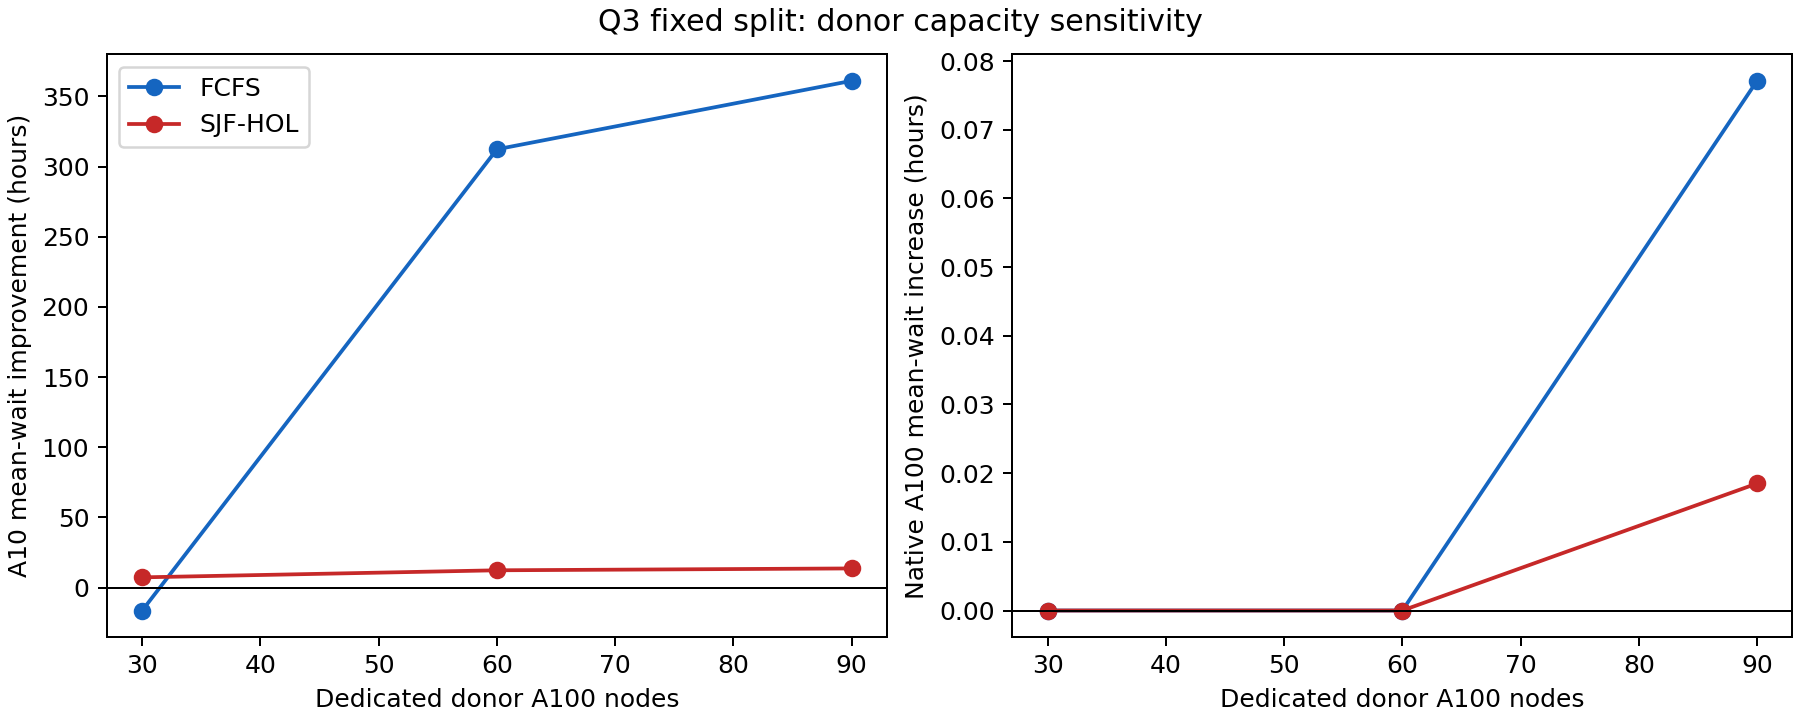
\includegraphics[width=0.86\linewidth]{figures/q3_donor_capacity_wait_tradeoff.png}\caption{Historical donor-capacity sensitivity. The left panel is A10 mean-wait change; the right panel is native A100 mean-wait change, with separate scales.}
\label{fig:r2q3tradeoff}\end{figure}

The historical sensitivity retains its negative cases: at 60 donors, 20\% routing raises FCFS A10 mean wait to 1,010.136 h and its maximum to 5,445.367 h; 30 donors at 10\% gives 916.407 h, worse than No substitution. For the 90-donor case, SPT-HOL native A100 has 2,150 positive-delay jobs, mean additional wait 0.018492 h over all 80,877 native jobs, and harmed-subgroup mean 0.695606 h. These finite paired results expose the management choice between A10 relief, native harm, tail, and completion count.

A financial extension is optional rather than a second experiment. If a tenant values completion time at $v$ per hour and pays $P$, voluntary substitution requires payment reduction at least $v$ times the completion-time increase. No price, participation rate, revenue, or profitability is inferred here. An online completion-cost routing rule is future work; no additional batch policy or borrowed threshold is introduced.
